\documentclass{article}
\usepackage{graphicx}
\begin{document}
	{\underline{\textbf{PROGRAMMING LANGUAGES:{ A HISTORICAL VIEW}}}}\\
	\center{\textbf{COBOL, JAVASCRIPT, PYTHON, FORTRAN, BASIC}}
	\newpage
	\section{FORTRAN}
	In late 1953, John W Backus proposed the idea of creating a more practical language than assembly language to his superiors at IBM (International Business Machines Corporation) for programming their IBM mainframe computer because the use of assembly language to write a code to represent complex calculations was a difficult and tiring process.
	IBM listened to his proposal and after 3 years in 1956, created Fortran, the worlds first programming language. 
	It was finally released in 1957
	
	\newpage
	In November 1954, the draft specifications of the IBM mathematical FORmular TRANslating system was finished. This is the first formal proposal for the language FORTRAN
	
	In the month of October of 1956, the first manual for FORTRAN introduced 
	
	On April 1954, the first FORTRAN compiler was made
	
	FORTRAN is mostly used by scientists and mathematicians for writing programs mostly dealing with numbers but it is not as popularly used for business purposes as opposed to COBOL\\
\newpage
	\begin{figure}
	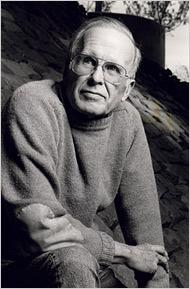
\includegraphics[width=0.7\linewidth]{john-w-backus}
	\caption{Image of the FORTRAN creator John W Backus }
	\label{fig:john-w-backus}
\end{figure}

\newpage
\textbf{APPLICATION EXAMPLES}
\begin{enumerate}
	\item HEC-RAS U.S. Army Corps of Engineers 1991 River Channel Water\\
	\item MODFLOW USGS 1983 3D Ground-water flow model\\
	\item ANSYS Dr. John Swanson 1970 finite element analysis, structural
	analysis\\
\end{enumerate}

\newpage
\underline{RELATED PROGRAMMING LANGUAGES}
\begin{enumerate}
	\item C++
	\item C
	\item F sharp
\end{enumerate}

\underline{AVAILABLE INTEGRATED DEVELOPMENT ENVIRONMENT (IDEs)}
\begin{enumerate}
\item Eclipse-Photran Photran
\end{enumerate}

\newpage
\section{\underline{cobol}}
Cobol was designed in 1959. Grace hopper, inventor of FLOW-MATIC, CODASYL ( the committee on data systems language), the American National Standards Institute (ANSI) and The International Organization for Standardization (ISO) assisted in developing the language.

At that time, the cost of programming was increasing fast and becoming very expensive so on April 8 1959, Mary K Hawes called a formal meeting to address the issue on common business languages. The meeting consisted of Grace Hoper, Saul Gorn and Jean Sammet.

They then requested for help from the department of defense (DOD) to sponsor  them in making a new language for business. Charles A. Philips, director of the data system research staff at the DOD, listened and agreed with their idea and decided to sponsor them.

Cobol was designed by Grace Hopper, Norman Discount, Jean E. Sammet, Howard Bromberg, William Seldon, Gertrude Tierney, Vernon Reeves,  with indirect reference to Grace Hoppers FLOW-MATIC\\
\newpage
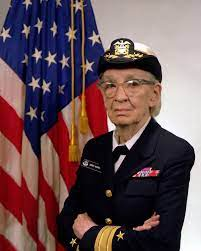
\includegraphics{grace hopper.jpg}
{Grace Hopper}

\newpage
\underline{APPLICATIONS}\\
          COBOL is used in finance, business, and
          administrative systems for companies and governments

\underline{SIMILAR LANGUAGES}\\
\begin{enumerate}
	\item Python
	\item C
	\item Java
\end{enumerate}

\newpage
\section{\textbf{PYTHON}}
Python, arguably the most commonly used programming language, was developed later in the 1980s by Guido van Rossum at Centrum Wiskunde and Informatica (CWI) in Netherland. 
Guido van Rossum, who helped in developing the ABC programming lang  uage, decided that ABC had some issues but he liked most of its features so he decided to fix the issues it had and create a better scripting language. He named the new and improved language Python gotten from a show he really liked called ‘Monty Python’s Flying Circus’.
The language was then released in 1991


\newpage
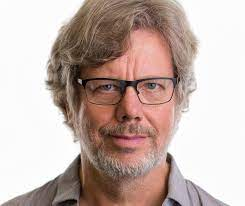
\includegraphics{guido.jpg}
{Guido Van Rossum}
\newpage

\underline{APPLICATIONS}

\begin{enumerate}
\item Dropbox
\item Django
\item Scify
\item Flask
\end{enumerate}


\underline{Similar languages}

\begin{enumerate}
	\item JavaScript
	\item Java
	\item PHP
	\item Anaconda
	
\end{enumerate}

\underline{IDE}

\begin{itemize}
	\item PyCharm
	\item Integrated Development Environment {IDLE}
	\item Spyder
	\item Eclipse
\end{itemize}

\newpage
\section{\textbf{JavaScript}}
JavaScript was crested in 1995 by Brendan Eich while he was at Netscape Communications.
In 1994, Netscape Navigator was released and quickly became a very popular browser. Then, only static webpages were possible so to fix that, they added a scripting language to their Navigator. 
Netscape then hired Brendan Eich to create a new language less like other languages and similar to Java. It was first called LiveScript but then changed to JavaScript.

\newpage
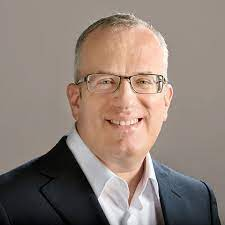
\includegraphics{Brendan Eich.jpg}
{Brendan Eich}
\newpage
\underline{APPLICATIONS}
\begin{enumerate}
	\item Candy Crush
\item Facebook 
\item linkedIn
\end{enumerate}

\underline{SIMILAR LANGUAGES}
\begin{enumerate}
	\item Python
	\item Java
	\item Typescript
	\item Ruby
\end{enumerate}

\underline{IDEs}
\begin{enumerate}
	\item WebStorm
    \item Eclipse
	\item NetBeans
	\item Komodo Edit
	\end{enumerate}

\newpage
\section{\underline{BASIC}}
BASIC (Beginners' All-purpose Symbolic Instruction Code) was created by Thomas Eugene Kurtz  and John George Kemeny who were mathematicians at Darmouth to help teach undergraduates in the mid 1960s. It was developed to allow students to write simple computer programs and was initially based on FORTRAN II
Dartmouth and Kurtzas developed a time sharing system called Dartmouth time sharing system DTSS for short. They then simplified the interface so that it could be easily used by students but since writing programs want easy Kurtzas tried simplifying existing languages until they came to the conclusion to create a completely new language. That’s how BASIC came to be. 

\newpage
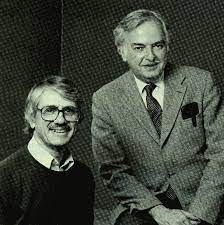
\includegraphics{basic guys.jpg}
{Thomas Eugene Kurtz  and John George Kemeny}
\newpage
\underline{APPLICATIONS}
\begin{itemize}
	\item Microsoft Basic
	\item BASIC A+
	\end{itemize}

\underline{SIMILAR LANGUAGES}
\begin{itemize}
\item Gambas
\item FreeBasic
\item 83 PureBasic
\item QB64
\end{itemize}

\underline{IDEs}
\begin{itemize}
\item Geany
\item Microsoft \item Visual c++
\item MonoDevelop
\item SharpDevelop
\end{itemize}

\newpage

\includegraphics{thanks.jpg}

	\end{document}